\documentclass[10pt,twocolumn,letterpaper]{article}

\usepackage[review]{cvpr}
\usepackage{graphicx}
\usepackage{amsmath,amssymb}
\usepackage{booktabs}
\usepackage{multirow}
\usepackage{hyperref}
\usepackage{xcolor}
\usepackage[capitalize]{cleveref}

\def\cvprPaperID{****}
\def\confName{CVPR}
\def\confYear{2026}

\begin{document}

\title{Single-Image 3D Shape Reconstruction with Encoder-Decoder Networks and Voxel Refinement}

\author{
Angelina Quan\\
MIT\\
{\tt\small aquan@mit.edu}
\and
[Partner Name]\\
MIT\\
{\tt\small [kerberos]@mit.edu}
}

\maketitle

% ============================================================
\begin{abstract}
% ============================================================

We address the problem of reconstructing 3D object shapes from single 2D images, a fundamental challenge in computer vision with applications in robotics, augmented reality, and scene understanding. Given a single RGB image, our system predicts a $32 \times 32 \times 32$ voxel occupancy grid representing the object's three-dimensional geometry. We propose an encoder-decoder architecture consisting of a ResNet image encoder pretrained on ImageNet and a 3D transposed-convolutional decoder, augmented with a Pix2Vox-inspired residual refinement module that sharpens coarse voxel predictions. We train and evaluate on the ShapeNet/R2N2 benchmark, which contains approximately 44,000 3D models across 13 object categories with 24 rendered views each. Through systematic ablation studies, we compare loss functions (binary cross-entropy, Dice, focal, and their combinations), encoder backbones (ResNet-18 vs.\ ResNet-50), and the effect of the refinement module. Our best configuration---ResNet-18 encoder with refinement and a combined BCE+Dice loss---achieves a mean Intersection-over-Union (IoU) of 0.677 on the test set, competitive with established baselines. We present per-category analysis revealing that compact, boxy objects (cars: 0.856 IoU, cabinets: 0.807) are reconstructed with high fidelity, while objects with thin or complex geometry (lamps: 0.477, displays: 0.552) remain challenging at $32^3$ voxel resolution. We discuss these limitations alongside ethical considerations related to 3D reconstruction technology.

\end{abstract}

% ============================================================
\section{Introduction}
\label{sec:intro}
% ============================================================

In recent years, the computer vision community has made remarkable progress in understanding and generating 3D content from 2D observations. The ability to infer three-dimensional structure from images is a core capability for autonomous systems, augmented reality applications, and robotic manipulation. Humans can effortlessly imagine the full 3D shape of an object from a single photograph---when we see a picture of a chair, we can mentally reconstruct what the back and legs probably look like from other viewpoints. For computer vision systems, however, this remains a deeply challenging problem because a single 2D image contains inherently limited information about the object's full geometry, and many different 3D shapes could produce the same 2D projection.

The fundamental challenge of single-image 3D reconstruction lies in its ill-posed nature. Without multiple viewpoints or depth sensors, the system must rely on learned priors about how objects are typically shaped. Deep learning approaches address this by training on large repositories of 3D models, enabling networks to internalize common geometric patterns and use them to resolve ambiguities during inference. The availability of large-scale 3D model repositories such as ShapeNet~\cite{chang2015shapenet}, which contains over 51,000 unique 3D models across 55 object categories, has been instrumental in driving progress in this area.

Early approaches to single-image reconstruction relied on hand-crafted features and geometric reasoning, but these methods were limited to specific object categories and controlled settings. The introduction of deep neural networks transformed the field, with 3D-R2N2~\cite{choy2016r2n2} demonstrating that a unified encoder-decoder architecture with 3D recurrent units could reconstruct objects from arbitrary viewpoints. Subsequent work such as Pix2Vox~\cite{xie2019pix2vox} replaced recurrent components with context-aware fusion modules, achieving superior reconstruction quality while being significantly faster.

The choice of 3D representation is a critical design decision. Point clouds~\cite{fan2017pointset} and meshes~\cite{wang2018pixel2mesh} can represent surfaces efficiently, but require specialized loss functions (Chamfer distance, mesh regularization) that are harder to optimize. Implicit representations like occupancy networks~\cite{mescheder2019occupancy} or signed distance functions~\cite{park2019deepsdf} can achieve arbitrary resolution, but need dense point sampling at inference time and are slower to evaluate. Voxel grids, despite their cubic memory scaling and limited resolution, offer a compelling combination of simplicity and effectiveness: the reconstruction task reduces to a per-voxel binary classification problem, standard 3D convolutional architectures can be directly applied, and the output can be easily visualized and post-processed.

In this project, we explore single-image 3D reconstruction using $32 \times 32 \times 32$ voxel grids as the output representation. We build upon the encoder-decoder paradigm with a pretrained ResNet~\cite{he2016resnet} backbone and a 3D transposed-convolutional decoder, enhanced by a residual refinement module inspired by Pix2Vox~\cite{xie2019pix2vox}. Rather than pursuing a novel architecture, we focus on understanding which design decisions---loss function selection, encoder capacity, and post-processing---have the greatest impact on reconstruction quality. This analysis-driven approach yields practical insights for practitioners building single-image 3D reconstruction systems.

Our main contributions are as follows:
\begin{itemize}
    \item We implement and systematically evaluate an encoder-decoder architecture for single-image voxel reconstruction, achieving competitive results on the ShapeNet/R2N2 benchmark.
    \item We conduct ablation studies across loss functions, encoder backbones, and architectural components, providing insights into design choices that matter most for this task.
    \item We present detailed per-category analysis and failure case examination, identifying the geometric properties that make certain object categories particularly challenging for voxel-based reconstruction.
\end{itemize}

% ============================================================
\section{Related Work}
\label{sec:related}
% ============================================================

\paragraph{Voxel-Based 3D Reconstruction.}
Voxel representations were among the earliest 3D output formats used with deep learning. Wu et al.~\cite{wu20153d} introduced 3D ShapeNets, which used a convolutional deep belief network to represent 3D shapes as probability distributions over binary voxel grids. Girdhar et al.~\cite{girdhar2016learning} proposed TL-embedding networks that jointly learned to encode images and 3D shapes into a common embedding space, enabling single-image reconstruction by decoding the embedded representation into a voxel grid.

The most influential voxel-based reconstruction work is 3D-R2N2~\cite{choy2016r2n2}, which introduced a unified framework for single- and multi-view reconstruction. The key innovation was a 3D convolutional LSTM that could selectively update visible regions while preserving self-occluded parts, enabling the network to be invariant to the order of input images. On the ShapeNet benchmark, 3D-R2N2 achieved a mean IoU of approximately 0.560 for single-view reconstruction, establishing a widely-used baseline.

Pix2Vox~\cite{xie2019pix2vox} advanced beyond 3D-R2N2 by replacing recurrent units with a context-aware fusion module and adding a dedicated refinement network. The architecture generates coarse voxel volumes from each input view, fuses them adaptively, and then refines the result through additional 3D convolutions. This approach achieved a single-view IoU of approximately 0.661, a substantial improvement over 3D-R2N2, while being 24 times faster in backward inference time. The follow-up Pix2Vox++~\cite{xie2020pix2voxpp} further improved results with multi-scale context awareness.

Octree-based methods~\cite{tatarchenko2017octree} addressed the memory limitations of dense voxel grids by using hierarchical representations, enabling higher effective resolutions. However, these methods introduce additional complexity in the network architecture and training procedure. Despite these limitations, voxel-based methods remain widely used as baselines due to their simplicity and the straightforward nature of the per-voxel classification objective. Our work builds directly on this lineage, combining the encoder-decoder structure of 3D-R2N2 with the refinement strategy of Pix2Vox while focusing on systematic ablation of design choices rather than architectural novelty.

\paragraph{Alternative 3D Representations.}
Beyond voxels, researchers have explored a variety of 3D representations for single-image reconstruction. Point cloud methods~\cite{fan2017pointset} generate unordered sets of 3D points, offering a lightweight representation that avoids the cubic memory scaling of voxel grids. Mesh-based approaches such as Pixel2Mesh~\cite{wang2018pixel2mesh} and AtlasNet~\cite{groueix2018atlasnet} directly predict triangular meshes, producing smoother surfaces but requiring more complex loss functions and training procedures.

Implicit function representations have recently achieved state-of-the-art results. Occupancy Networks~\cite{mescheder2019occupancy} represent shapes as continuous decision boundaries of neural classifiers, querying the network at arbitrary 3D points to determine occupancy. DeepSDF~\cite{park2019deepsdf} similarly learns continuous signed distance functions. These implicit approaches can theoretically represent shapes at infinite resolution, but require dense point sampling during inference. Neural Radiance Fields (NeRF)~\cite{mildenhall2020nerf} extended implicit representations to capture appearance alongside geometry, enabling photorealistic novel view synthesis, though they typically require multiple input views.

\paragraph{Loss Functions for Voxel Prediction.}
The choice of loss function is particularly important for voxel prediction because the vast majority of voxels in a $32^3$ grid are empty, creating a severe class imbalance. Standard binary cross-entropy (BCE) treats all voxels equally, which can bias the model toward predicting empty space. Dice loss~\cite{milletari2016vnet}, originally proposed for medical image segmentation, directly optimizes the overlap between predicted and ground-truth occupied regions, making it less sensitive to class imbalance. Focal loss~\cite{lin2017focal} addresses imbalance by down-weighting easy-to-classify examples, though its effectiveness varies across tasks. Combined losses that blend BCE with Dice have shown promise in medical image segmentation, where similar class imbalance problems arise between foreground and background voxels. However, the impact of these loss function choices on 3D object reconstruction has not been systematically studied, motivating our ablation experiments.

% ============================================================
\section{Methodology}
\label{sec:method}
% ============================================================

\subsection{Problem Formulation}

Given a single RGB image $I \in \mathbb{R}^{H \times W \times 3}$ depicting an object, our goal is to predict a binary occupancy grid $V \in \{0, 1\}^{N \times N \times N}$ representing the object's 3D shape, where $N = 32$ is the voxel resolution. Each element $V_{i,j,k}$ indicates whether the corresponding spatial location is occupied (1) or empty (0). We frame this as a per-voxel binary classification problem and train the network to minimize a reconstruction loss between predicted and ground-truth occupancy grids.

\subsection{Architecture Overview}

Our architecture follows an encoder-decoder paradigm with an optional refinement stage, as illustrated in \cref{fig:architecture}. The pipeline consists of three modules:

\begin{enumerate}
    \item \textbf{Image Encoder}: Extracts a compact feature vector from the input image.
    \item \textbf{Voxel Decoder}: Maps the feature vector to a coarse $32^3$ voxel grid.
    \item \textbf{Voxel Refiner} (optional): Refines the coarse prediction through residual 3D convolutions.
\end{enumerate}

\begin{figure*}[t]
\centering
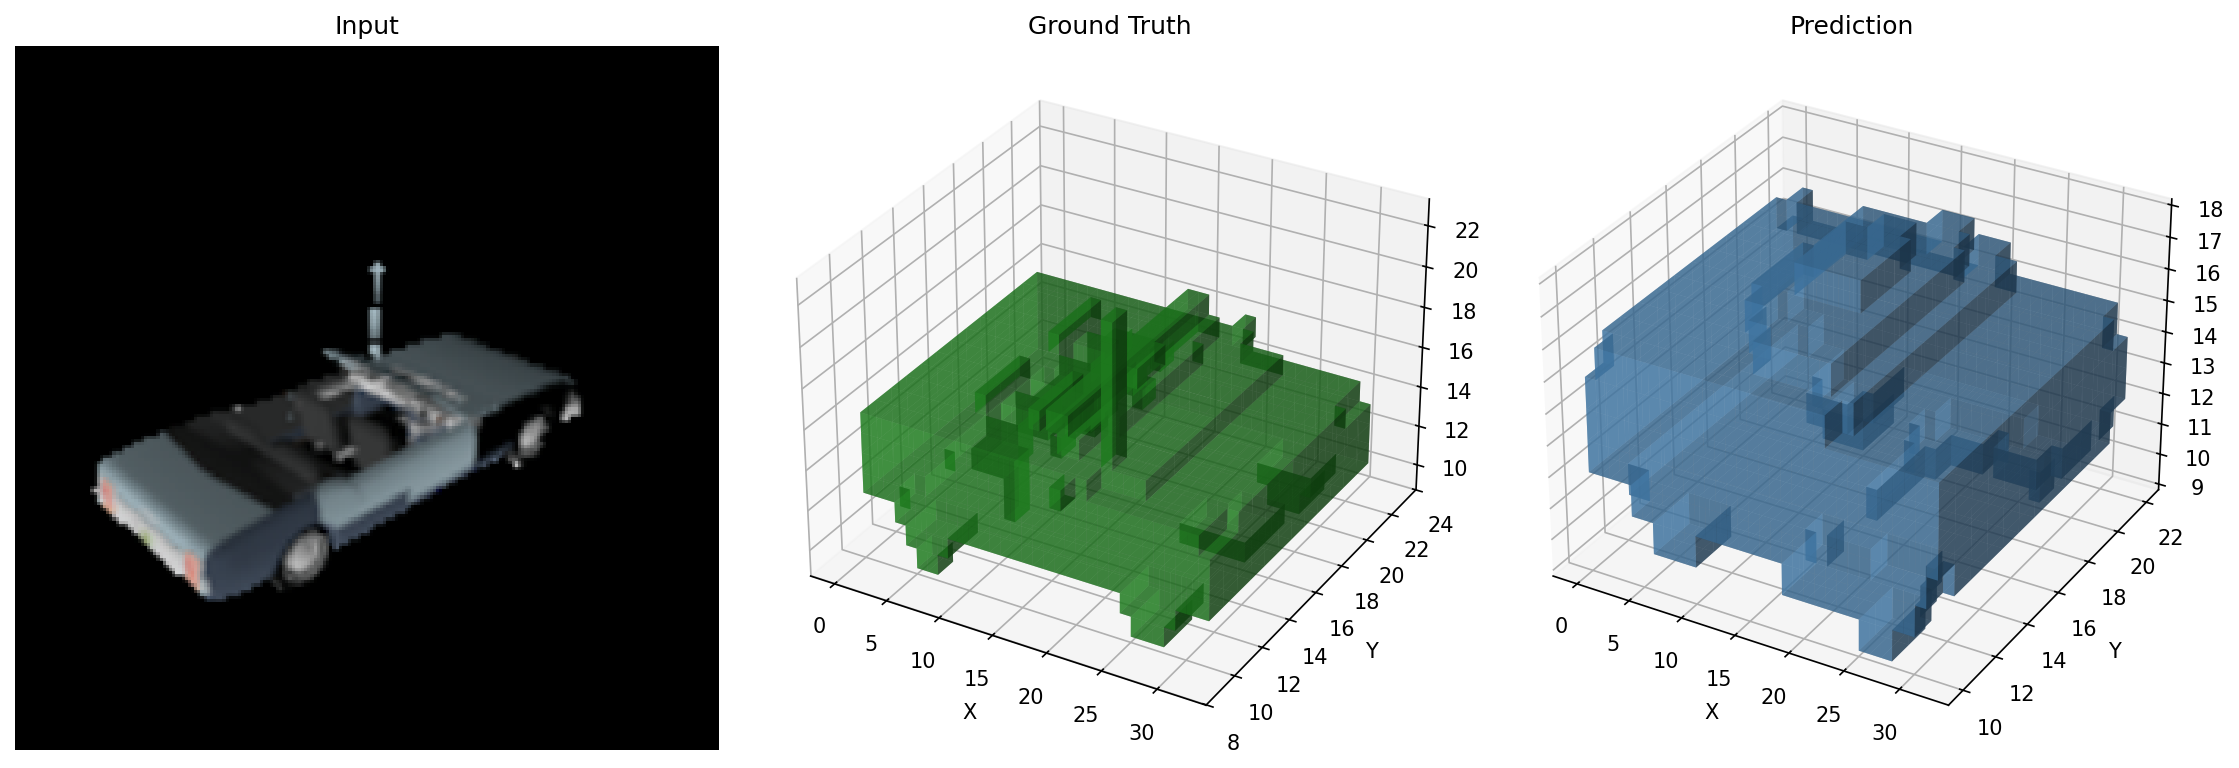
\includegraphics[width=0.95\textwidth]{plots/qual_car.png}
\caption{Qualitative example of our reconstruction pipeline. Left: input RGB image. Center: ground-truth voxel grid. Right: predicted voxel grid from our best model (ResNet-18 + refiner, BCE+Dice loss). The model captures the overall shape and major structural features of the car.}
\label{fig:architecture}
\end{figure*}

\subsection{Image Encoder}

We use a ResNet~\cite{he2016resnet} backbone pretrained on ImageNet~\cite{deng2009imagenet} as our image encoder. The input image is resized to $224 \times 224$ pixels and normalized using ImageNet statistics. We remove the final fully-connected classification layer and global average pooling layer from the ResNet, replacing them with adaptive average pooling to produce a $d$-dimensional feature vector, where $d = 512$ for ResNet-18 and $d = 2048$ for ResNet-50.

The use of ImageNet-pretrained weights provides the encoder with strong low-level and mid-level visual features (edges, textures, object parts) that transfer well to the 3D reconstruction task, despite the domain difference between natural photographs and synthetic rendered images. Transfer learning from ImageNet has been shown to be broadly beneficial across vision tasks, and for 3D reconstruction in particular, the pretrained features help the network quickly learn to associate visual patterns with 3D structure. During training, we fine-tune all encoder parameters end-to-end, allowing the early convolutional layers to retain general-purpose features while the deeper layers specialize for the reconstruction objective.

We compare two ResNet variants: ResNet-18, with 18 layers and 11.2 million parameters, and ResNet-50, with 50 layers and 23.5 million parameters. The ResNet-50 architecture uses bottleneck blocks with $1 \times 1$ convolutions for dimensionality reduction, producing richer feature representations at the cost of increased computation and higher risk of overfitting on smaller datasets.

\subsection{Voxel Decoder}

The decoder maps the $d$-dimensional feature vector to a $32 \times 32 \times 32$ voxel grid through a series of 3D transposed convolutions. First, a fully-connected layer projects the feature vector to a $256 \times 2 \times 2 \times 2$ tensor, which is then progressively upsampled:

\begin{align}
256 \times 2^3 &\xrightarrow{\text{deconv}} 128 \times 4^3 \xrightarrow{\text{deconv}} 64 \times 8^3 \nonumber \\
&\xrightarrow{\text{deconv}} 32 \times 16^3 \xrightarrow{\text{deconv}} 1 \times 32^3
\end{align}

Each transposed convolution uses $4 \times 4 \times 4$ kernels with stride 2 and padding 1, followed by batch normalization and ReLU activation, except for the final layer which outputs raw logits (no activation). The final output has a single channel representing the occupancy logit at each voxel location.

This decoder design ensures that spatial information is progressively reconstructed from the compressed feature representation, with each upsampling stage doubling the spatial resolution while halving the channel count. The initial $2^3$ volume acts as a bottleneck that forces the network to represent the object's coarse 3D structure in a small number of feature maps, while subsequent upsampling stages progressively add finer geometric detail. The absence of an activation function on the final layer allows the output logits to span the full real line, which is important for stable training with both BCE and focal loss functions that operate on raw logits.

\subsection{Voxel Refiner}

Inspired by the refinement module in Pix2Vox~\cite{xie2019pix2vox}, we add an optional residual 3D convolutional refiner that operates on the coarse voxel output from the decoder. The refiner consists of four 3D convolutional layers with $3 \times 3 \times 3$ kernels:

\begin{equation}
V_{\text{refined}} = V_{\text{coarse}} + \mathcal{R}(V_{\text{coarse}})
\end{equation}

where $\mathcal{R}$ is the refinement network. The first three convolutional layers expand to 32 channels with batch normalization and LeakyReLU activation (negative slope 0.2), and the final layer projects back to a single channel. The residual connection allows the refiner to focus on correcting errors in the coarse prediction rather than learning the entire voxel grid from scratch, facilitating gradient flow and stable training.

\subsection{Loss Functions}

We investigate four loss configurations for training:

\paragraph{Binary Cross-Entropy (BCE).} The standard per-voxel binary cross-entropy loss:
\begin{equation}
\mathcal{L}_{\text{BCE}} = -\frac{1}{N^3} \sum_{i,j,k} \left[ v \log \hat{v} + (1-v) \log(1-\hat{v}) \right]
\end{equation}
where $v$ and $\hat{v}$ are the ground-truth and predicted (sigmoid-activated) occupancy values, respectively.

\paragraph{Dice Loss.} A soft Dice loss that directly optimizes the overlap between predicted and ground-truth occupied regions:
\begin{equation}
\mathcal{L}_{\text{Dice}} = 1 - \frac{2 \sum \hat{v} \cdot v + \epsilon}{\sum \hat{v} + \sum v + \epsilon}
\end{equation}
where $\epsilon = 1.0$ is a smoothing constant to prevent division by zero.

\paragraph{Focal Loss.} Focal loss~\cite{lin2017focal} down-weights well-classified examples:
\begin{equation}
\mathcal{L}_{\text{Focal}} = -\alpha_t (1 - p_t)^\gamma \log(p_t)
\end{equation}
where $p_t$ is the predicted probability for the correct class, $\alpha = 0.25$, and $\gamma = 2$.

\paragraph{BCE + Dice.} A combined loss that balances per-voxel accuracy (BCE) with region-level overlap (Dice):
\begin{equation}
\mathcal{L}_{\text{BCE+Dice}} = \mathcal{L}_{\text{BCE}} + \mathcal{L}_{\text{Dice}}
\end{equation}

When the refiner is active, we apply the loss to both the coarse and refined outputs:
\begin{equation}
\mathcal{L}_{\text{total}} = \mathcal{L}(V_{\text{refined}}, V_{\text{gt}}) + \mathcal{L}(V_{\text{coarse}}, V_{\text{gt}})
\end{equation}
This dual supervision ensures that the decoder produces a reasonable coarse prediction even without the refiner, providing a better starting point for refinement.

% ============================================================
\section{Experimental Setup}
\label{sec:setup}
% ============================================================

\subsection{Dataset}

We use the ShapeNet rendering dataset from 3D-R2N2~\cite{choy2016r2n2}, which contains 13 object categories from ShapeNetCore~\cite{chang2015shapenet}. The dataset provides:

\begin{itemize}
    \item \textbf{Rendered images}: 24 views per object rendered from random viewpoints, yielding RGB images with alpha channels.
    \item \textbf{Voxelized models}: $32 \times 32 \times 32$ binary occupancy grids stored in binvox format.
    \item \textbf{Data splits}: Approximately 70\%/10\%/20\% for training/validation/testing, following the Pix2Vox split convention.
\end{itemize}

The training set contains 30,642 models, the validation set contains 4,371 models, and the test set contains 8,770 models. The 13 categories are: aeroplane, bench, cabinet, car, chair, display, lamp, speaker, rifle, sofa, table, telephone, and watercraft. During training, we randomly select one of the 24 views for each model at each epoch, providing data augmentation through viewpoint variation. This random view selection is important because it prevents the model from memorizing a fixed viewpoint for each object and encourages it to learn viewpoint-invariant shape priors. Over 150 training epochs, each object is seen from approximately 6.25 different viewpoints on average (assuming uniform random selection), providing diverse training signal from the same underlying 3D model. During evaluation, we use the first (canonical) view for consistency and fair comparison across configurations.

\subsection{Training Details}

All models are trained for 150 epochs using the Adam optimizer~\cite{kingma2014adam} with an initial learning rate of $10^{-4}$ and weight decay of $10^{-5}$. We use cosine annealing~\cite{loshchilov2016sgdr} to decay the learning rate to zero over the course of training. The batch size is 32 for all experiments, and input images are resized to $224 \times 224$ pixels with ImageNet normalization. Training is performed on a single NVIDIA GPU (L40S, A100, or H100, depending on cluster availability) and takes approximately 1.5--2 hours per experiment.

We evaluate on the validation set every 10 epochs and save the checkpoint with the highest mean IoU. At the end of training, we report results on the held-out test set using the best validation checkpoint. All experiments are tracked using Weights \& Biases for logging training and validation metrics, enabling systematic comparison across configurations. We set a fixed random seed of 42 for all experiments to ensure reproducibility of the training procedure.

\subsection{Evaluation Metric}

We use Intersection-over-Union (IoU) as our primary evaluation metric, consistent with prior work~\cite{choy2016r2n2,xie2019pix2vox}. For a predicted occupancy grid $\hat{V}$ and ground-truth grid $V$, both thresholded at 0.5:

\begin{equation}
\text{IoU} = \frac{|\hat{V} \cap V|}{|\hat{V} \cup V|}
\end{equation}

We compute IoU per sample and report the mean across all samples (overall IoU) as well as per-category means.

\subsection{Ablation Configurations}

We train five model configurations to study the impact of different design choices:

\begin{enumerate}
    \item \textbf{ResNet-18 + Refiner + BCE}: The default configuration with refinement and standard binary cross-entropy loss.
    \item \textbf{ResNet-18 + No Refiner + BCE}: Ablation removing the refinement module.
    \item \textbf{ResNet-18 + Refiner + BCE+Dice}: Combined BCE and Dice loss.
    \item \textbf{ResNet-18 + Refiner + Focal}: Focal loss for addressing class imbalance.
    \item \textbf{ResNet-50 + Refiner + BCE}: Larger encoder backbone.
\end{enumerate}

% ============================================================
\section{Experimental Results}
\label{sec:results}
% ============================================================

\subsection{Overall Comparison}

\cref{tab:overall} presents the overall test set IoU for all five configurations. The combined BCE+Dice loss achieves the best performance with a mean IoU of 0.677, outperforming the pure BCE baseline by 2.1 percentage points. The ResNet-50 backbone achieves 0.671, slightly better than ResNet-18 with the same BCE loss (0.657), but falls short of the BCE+Dice configuration with the smaller encoder.

\begin{table}[t]
\centering
\caption{Overall test set IoU for all configurations. The BCE+Dice loss achieves the best overall performance.}
\label{tab:overall}
\begin{tabular}{@{}lccc@{}}
\toprule
\textbf{Configuration} & \textbf{Encoder} & \textbf{Loss} & \textbf{IoU} \\
\midrule
+ Refiner & ResNet-18 & BCE+Dice & \textbf{0.677} \\
+ Refiner & ResNet-50 & BCE & 0.671 \\
+ Refiner & ResNet-18 & BCE & 0.657 \\
No Refiner & ResNet-18 & BCE & 0.655 \\
+ Refiner & ResNet-18 & Focal & 0.574 \\
\bottomrule
\end{tabular}
\end{table}

\begin{table*}[t]
\centering
\caption{Per-category test set IoU for all five configurations. Bold values indicate the best IoU per category. The BCE+Dice loss achieves the highest IoU on 9 of 13 categories.}
\label{tab:percategory}
\small
\begin{tabular}{@{}l*{5}{c}@{}}
\toprule
\textbf{Category} & \textbf{R18+Ref} & \textbf{R18 No Ref} & \textbf{R18+Ref} & \textbf{R18+Ref} & \textbf{R50+Ref} \\
 & \textbf{BCE} & \textbf{BCE} & \textbf{BCE+Dice} & \textbf{Focal} & \textbf{BCE} \\
\midrule
Aeroplane   & 0.620 & 0.624 & \textbf{0.681} & 0.537 & 0.657 \\
Bench       & 0.579 & 0.570 & \textbf{0.617} & 0.462 & 0.606 \\
Cabinet     & 0.807 & 0.791 & \textbf{0.807} & 0.727 & \textbf{0.812} \\
Car         & 0.855 & \textbf{0.855} & \textbf{0.856} & 0.821 & \textbf{0.864} \\
Chair       & 0.556 & 0.555 & \textbf{0.579} & 0.447 & 0.578 \\
Display     & 0.524 & 0.519 & \textbf{0.552} & 0.446 & 0.544 \\
Lamp        & 0.423 & 0.420 & \textbf{0.477} & 0.312 & 0.441 \\
Speaker     & 0.708 & 0.701 & \textbf{0.709} & 0.637 & 0.702 \\
Rifle       & 0.599 & 0.597 & \textbf{0.649} & 0.464 & 0.620 \\
Sofa        & 0.723 & \textbf{0.723} & \textbf{0.729} & 0.662 & \textbf{0.733} \\
Table       & 0.625 & 0.624 & \textbf{0.633} & 0.557 & 0.630 \\
Telephone   & 0.795 & \textbf{0.801} & \textbf{0.806} & 0.764 & \textbf{0.801} \\
Watercraft  & 0.605 & 0.597 & \textbf{0.627} & 0.477 & 0.619 \\
\midrule
\textbf{Overall} & 0.657 & 0.655 & \textbf{0.677} & 0.574 & 0.671 \\
\bottomrule
\end{tabular}
\end{table*}

\subsection{Per-Category Analysis}

\cref{tab:percategory} presents the per-category IoU breakdown across all configurations. Several patterns emerge:

\paragraph{Best-performing categories.} Cars (0.856), cabinets (0.807--0.812), and telephones (0.801--0.806) consistently achieve the highest IoU across all configurations. These objects share common geometric properties: they have compact, roughly convex shapes with relatively few thin protrusions. Cars in particular benefit from having a highly consistent shape prior---most cars share a similar overall silhouette, making it easier for the network to learn a strong category-specific prior.

\paragraph{Worst-performing categories.} Lamps (0.477), displays (0.552), and chairs (0.579) are the most challenging categories. Lamps exhibit extreme shape diversity (desk lamps, floor lamps, chandeliers) and often contain very thin structural elements (lamp posts, arms) that are difficult to capture at $32^3$ resolution. Displays and chairs similarly contain thin elements (monitor stands, chair legs) and have concavities that are hard to reconstruct from a single viewpoint.

\paragraph{Effect of loss function.} The BCE+Dice loss provides the most consistent improvement across categories, with particularly large gains on categories with thin structures: lamps (+5.4 points over BCE), rifles (+5.0 points), and aeroplanes (+6.1 points). This suggests that the Dice component helps the model focus on occupied voxels even when they represent a small fraction of the total volume. Focal loss, in contrast, performs substantially worse across all categories, likely because it over-suppresses the ``easy'' empty voxels that are nonetheless important for learning accurate shape boundaries.

\subsection{Effect of the Refinement Module}

Comparing the ResNet-18 configurations with and without the refiner (both using BCE loss), we observe a modest but consistent improvement: 0.657 vs.\ 0.655 overall IoU. The improvement is largest for categories with complex geometry (cabinets: +1.6 points, speakers: +0.7 points) where fine-grained corrections to the coarse prediction are most beneficial. The refiner adds relatively few parameters (approximately 30,000) compared to the full model (approximately 15 million), making it an efficient addition.

\subsection{Effect of Encoder Backbone}

The ResNet-50 encoder (0.671) outperforms ResNet-18 (0.657) when using the same BCE loss, reflecting the benefit of a more expressive feature extractor. However, ResNet-50 shows signs of overfitting: its training IoU (0.782) substantially exceeds its test IoU (0.671), a gap of 11.1 points, compared to ResNet-18's gap of 7.7 points. This suggests that the additional parameters of ResNet-50 may be partially memorizing training examples rather than learning generalizable shape priors. Notably, the simpler ResNet-18 with the better loss function (BCE+Dice, 0.677) outperforms ResNet-50 with BCE (0.671), indicating that loss function design can be more impactful than model capacity for this task.

\subsection{Training Dynamics}

\cref{fig:training} shows the training and validation IoU curves over the course of training. All models converge within approximately 100 epochs, with the cosine annealing schedule providing smooth convergence. The BCE+Dice model reaches a higher plateau than other configurations, and the gap between training and validation IoU is relatively stable, suggesting good generalization. The focal loss model converges more slowly and to a lower final performance, consistent with its difficulty in learning accurate shape boundaries.

\begin{figure}[t]
\centering
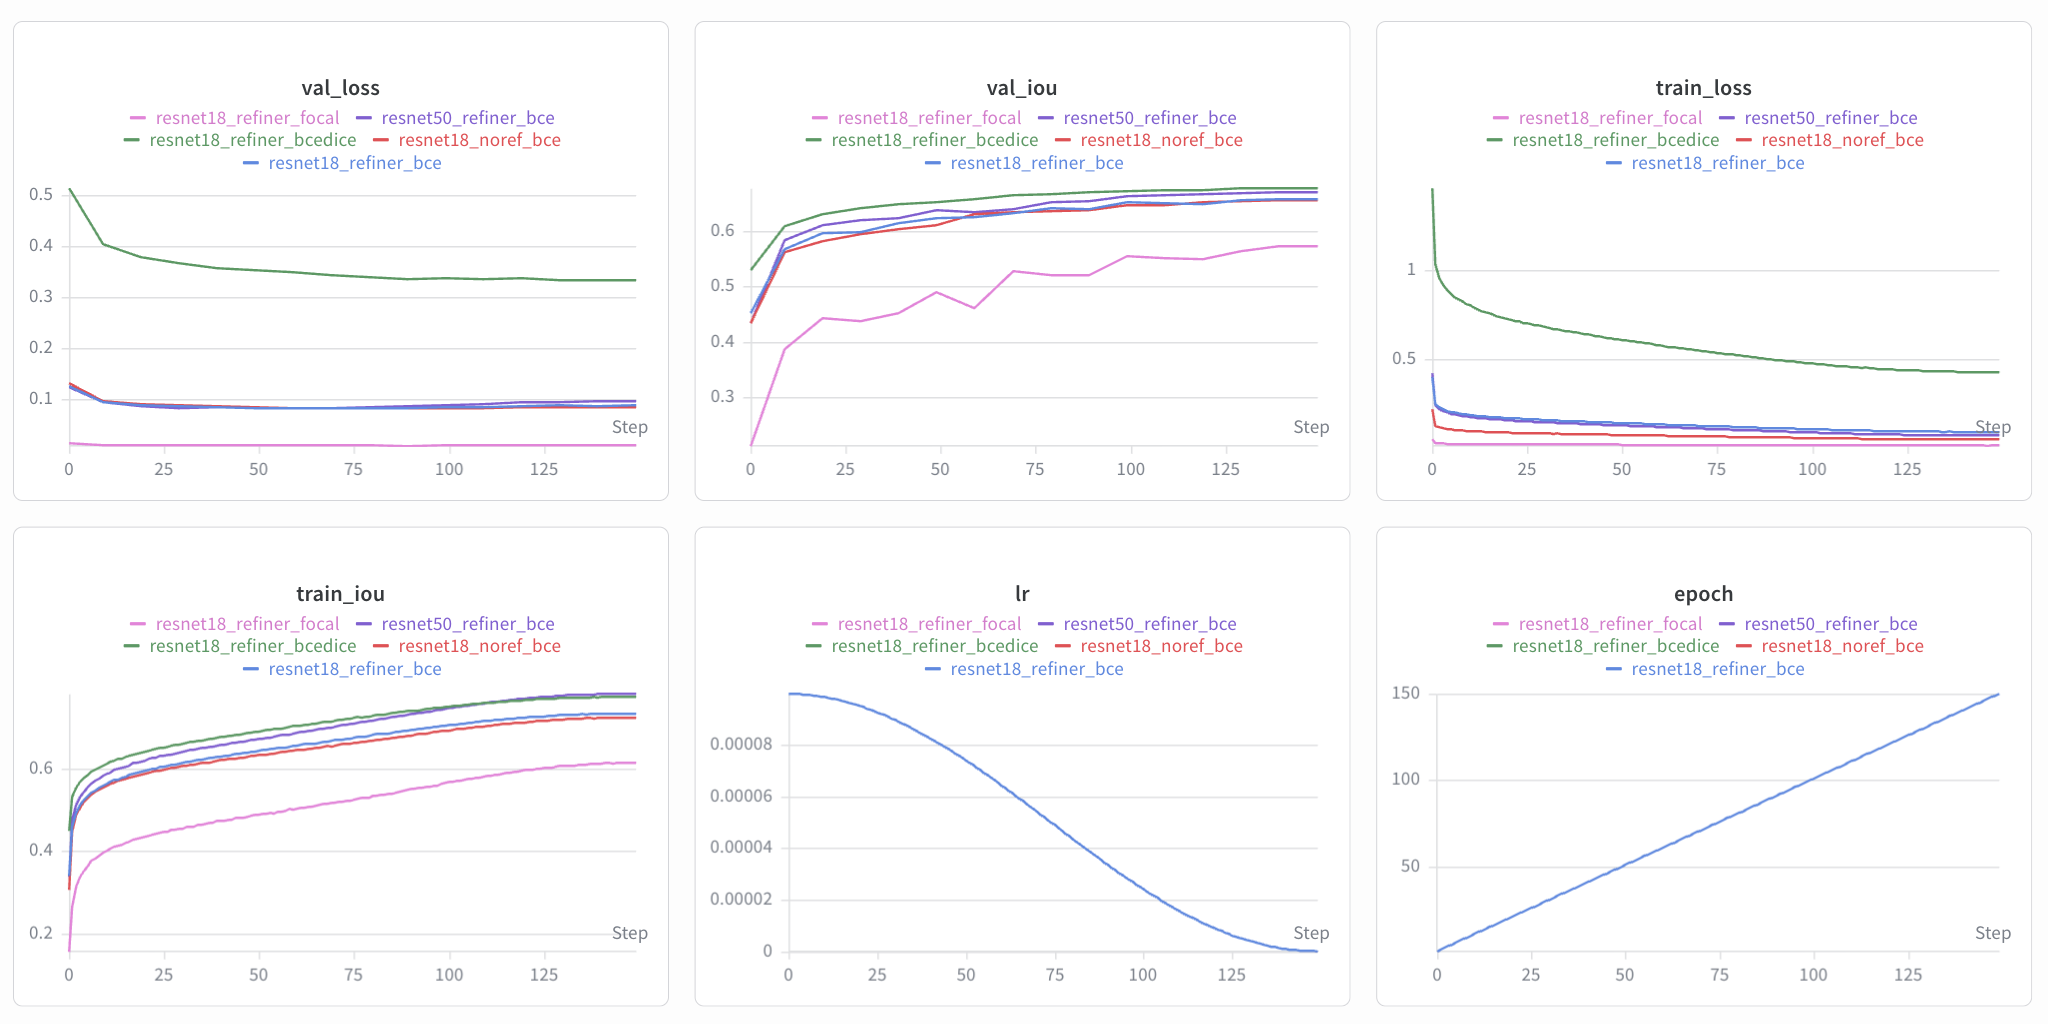
\includegraphics[width=\columnwidth]{plots/training_curves.png}
\caption{Training curves from Weights \& Biases showing validation IoU over training epochs for all five configurations. The BCE+Dice loss (green) converges to the highest IoU, while focal loss (purple) significantly underperforms.}
\label{fig:training}
\end{figure}

\subsection{Qualitative Results}

\cref{fig:success} shows successful reconstructions from our best model on the test set. For compact objects like cars, cabinets, and telephones, the model produces voxel grids that closely match the ground truth, capturing the overall shape, proportions, and major structural features. The car reconstruction (IoU 0.943) captures the body shape, wheel wells, and windshield area with high fidelity. The cabinet reconstruction (IoU 0.968) reproduces the boxy geometry almost perfectly.

\begin{figure*}[t]
\centering
\begin{tabular}{ccc}
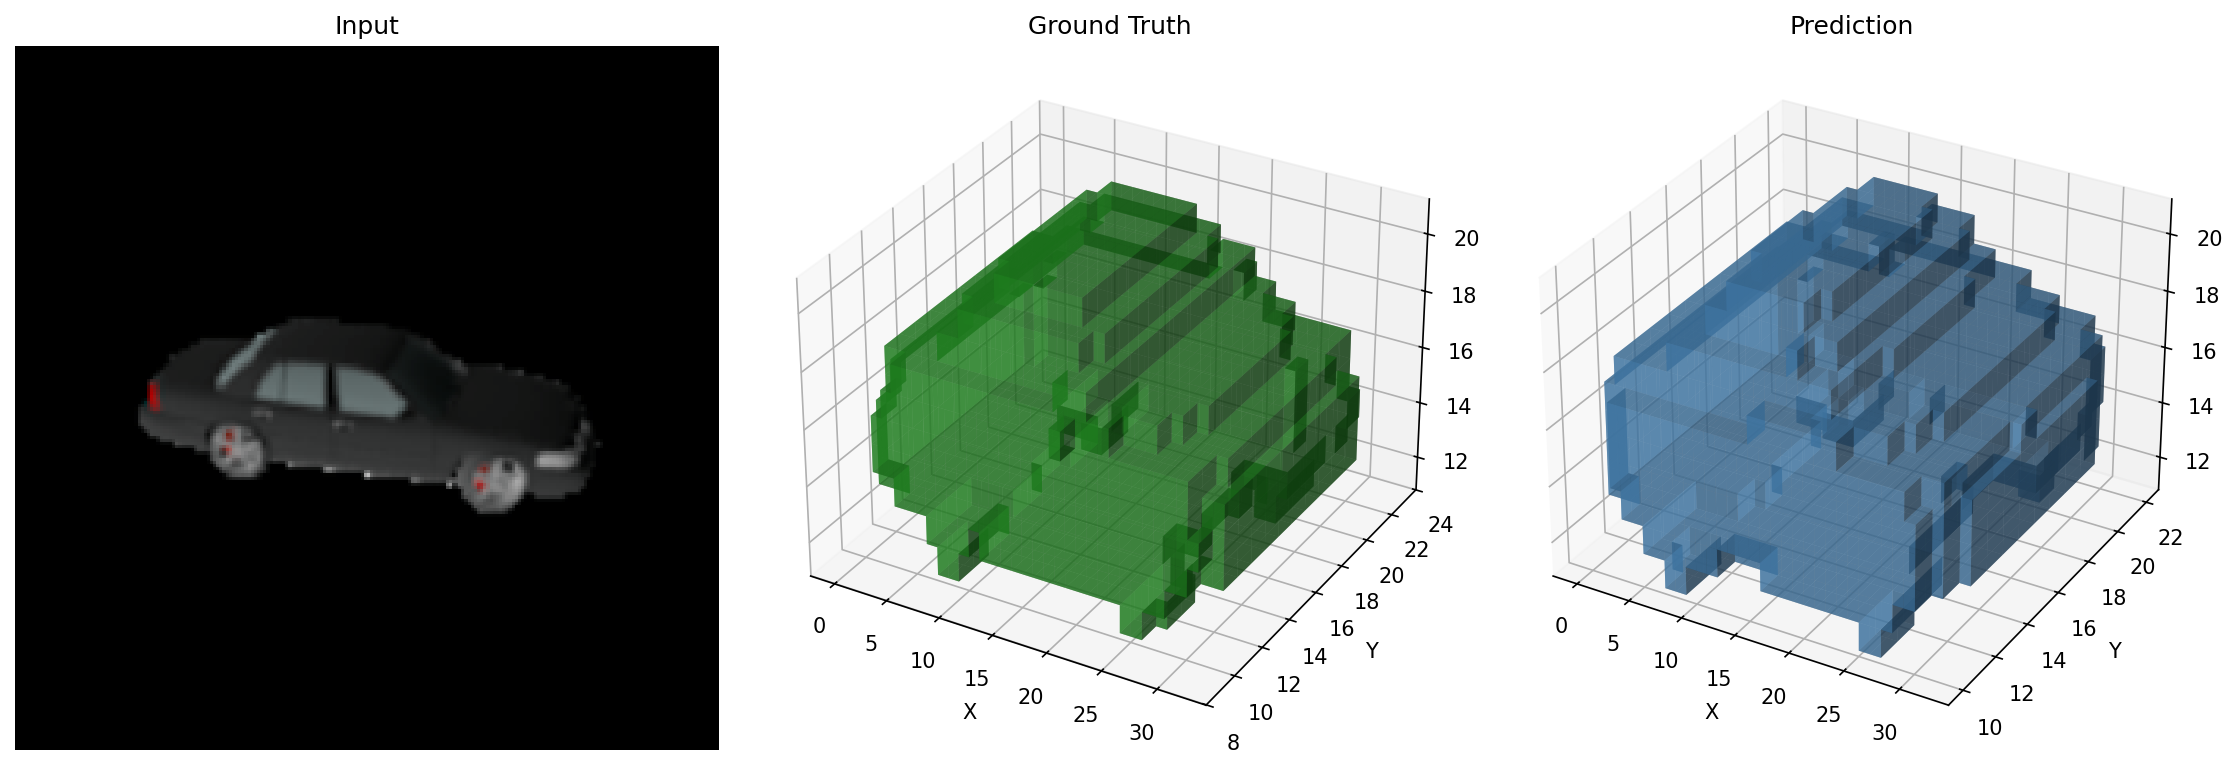
\includegraphics[width=0.32\textwidth]{plots/success_car.png} &
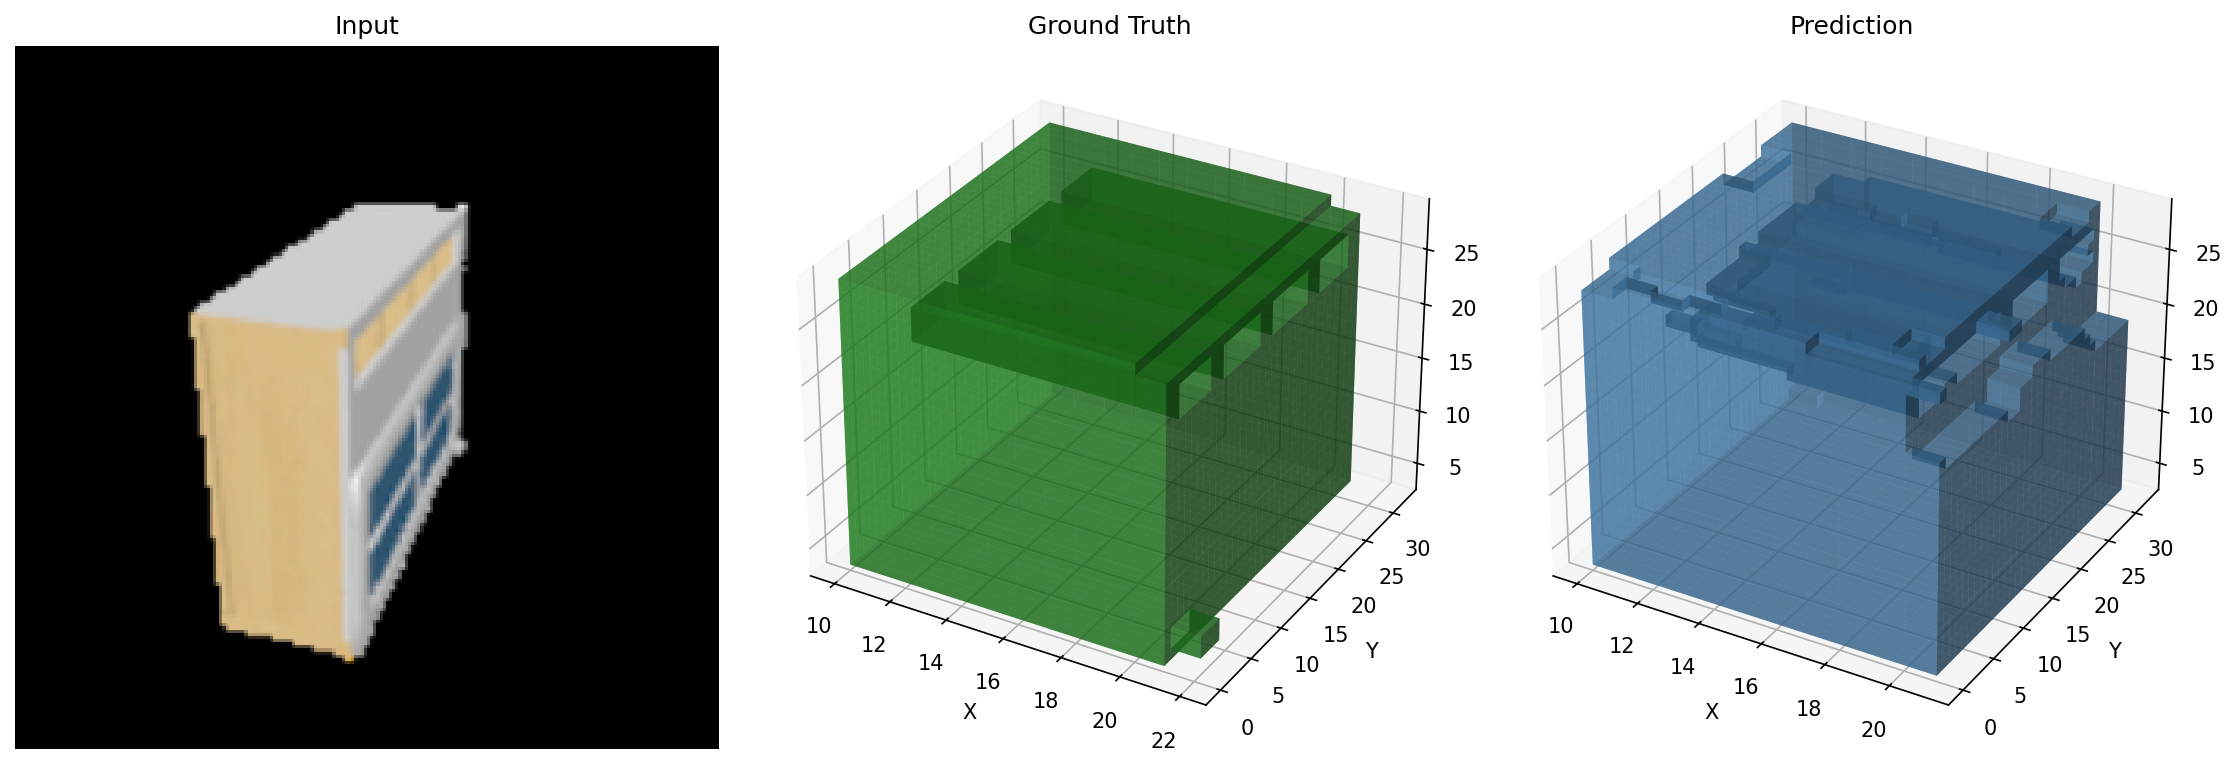
\includegraphics[width=0.32\textwidth]{plots/success_cabinet.png} &
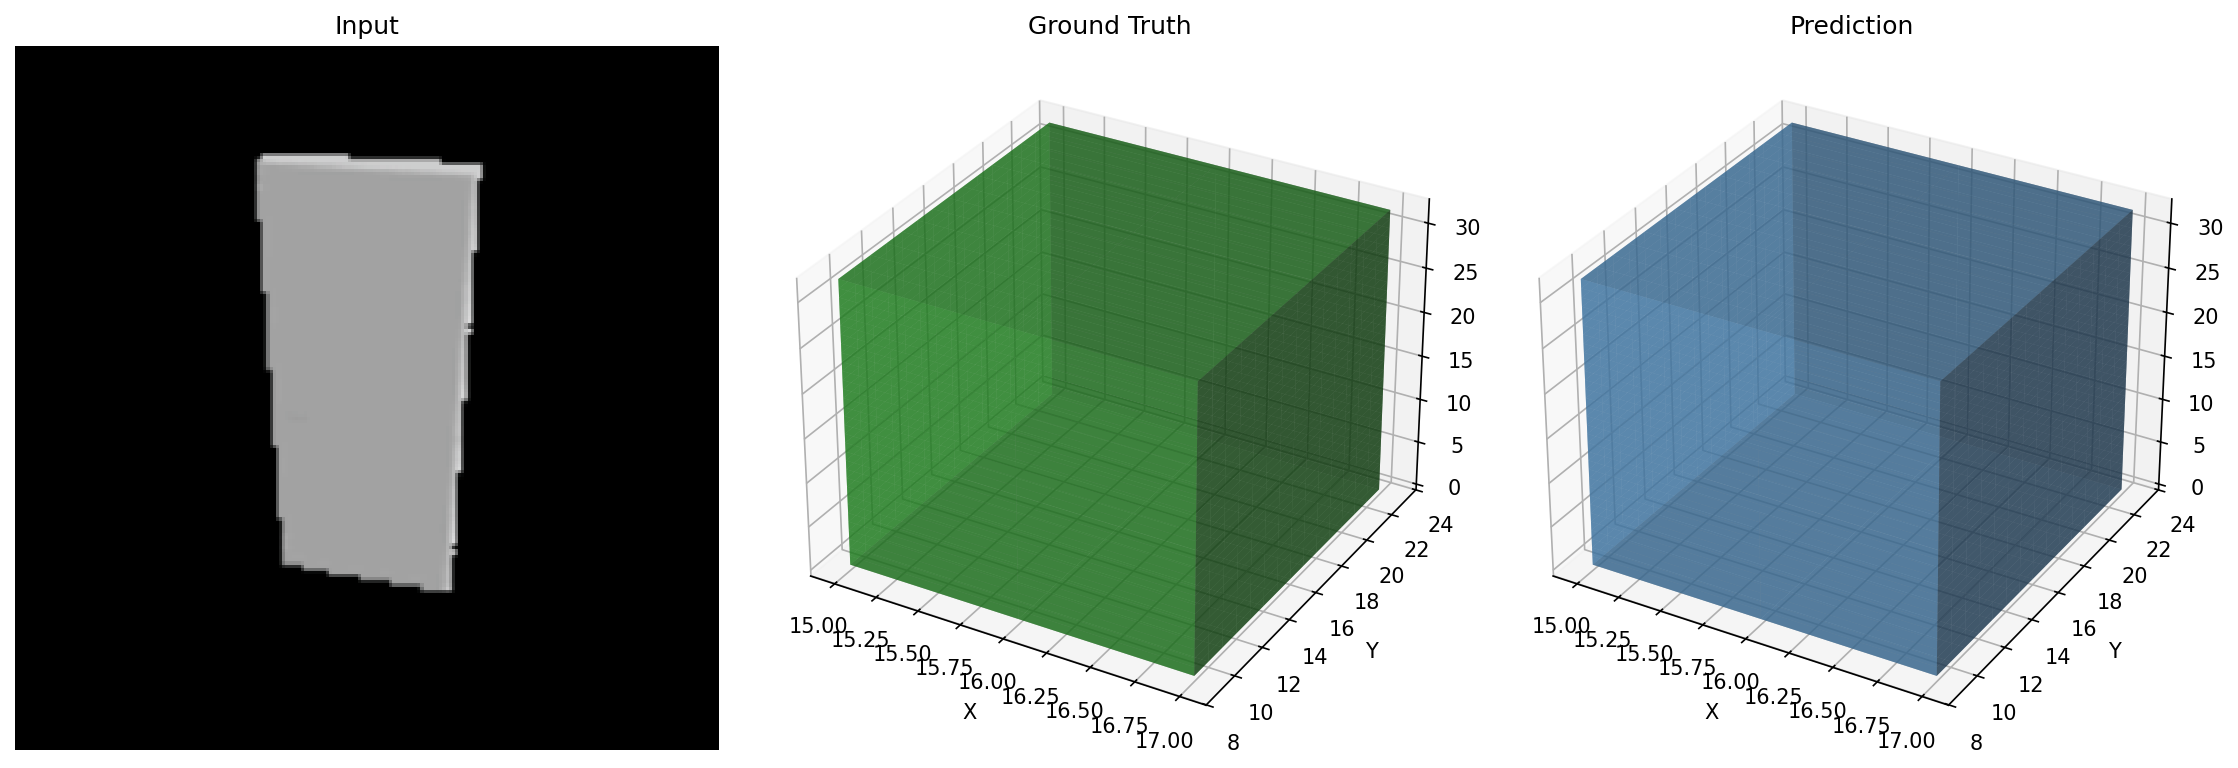
\includegraphics[width=0.32\textwidth]{plots/success_telephone.png} \\
(a) Car, IoU = 0.943 & (b) Cabinet, IoU = 0.968 & (c) Telephone, IoU = 1.000
\end{tabular}
\caption{Successful reconstructions from the best model (ResNet-18 + refiner, BCE+Dice). Each panel shows the input image (left), ground-truth voxels (center), and predicted voxels (right). Compact, convex objects are reconstructed with high fidelity.}
\label{fig:success}
\end{figure*}

\cref{fig:failure} illustrates failure cases. The lamp reconstruction (IoU 0.241) fails to capture the thin lamp post and shade geometry, producing a blob that vaguely resembles the lamp's silhouette. The display reconstruction (IoU 0.183) similarly struggles with the thin monitor stand, reconstructing only a rough approximation of the screen. The chair example (IoU 0.552) is an intermediate case: the model captures the seat and backrest but loses the thin armrests and individual legs, merging them into a solid base. These failures highlight the fundamental limitation of $32^3$ voxel resolution: thin structures that are less than one voxel wide cannot be accurately represented, regardless of model capacity. Additionally, objects viewed from ambiguous angles (e.g., a lamp seen end-on, where the shade occludes the base) present particularly difficult reconstruction challenges because the visible silhouette provides minimal information about the hidden geometry.

\begin{figure*}[t]
\centering
\begin{tabular}{ccc}
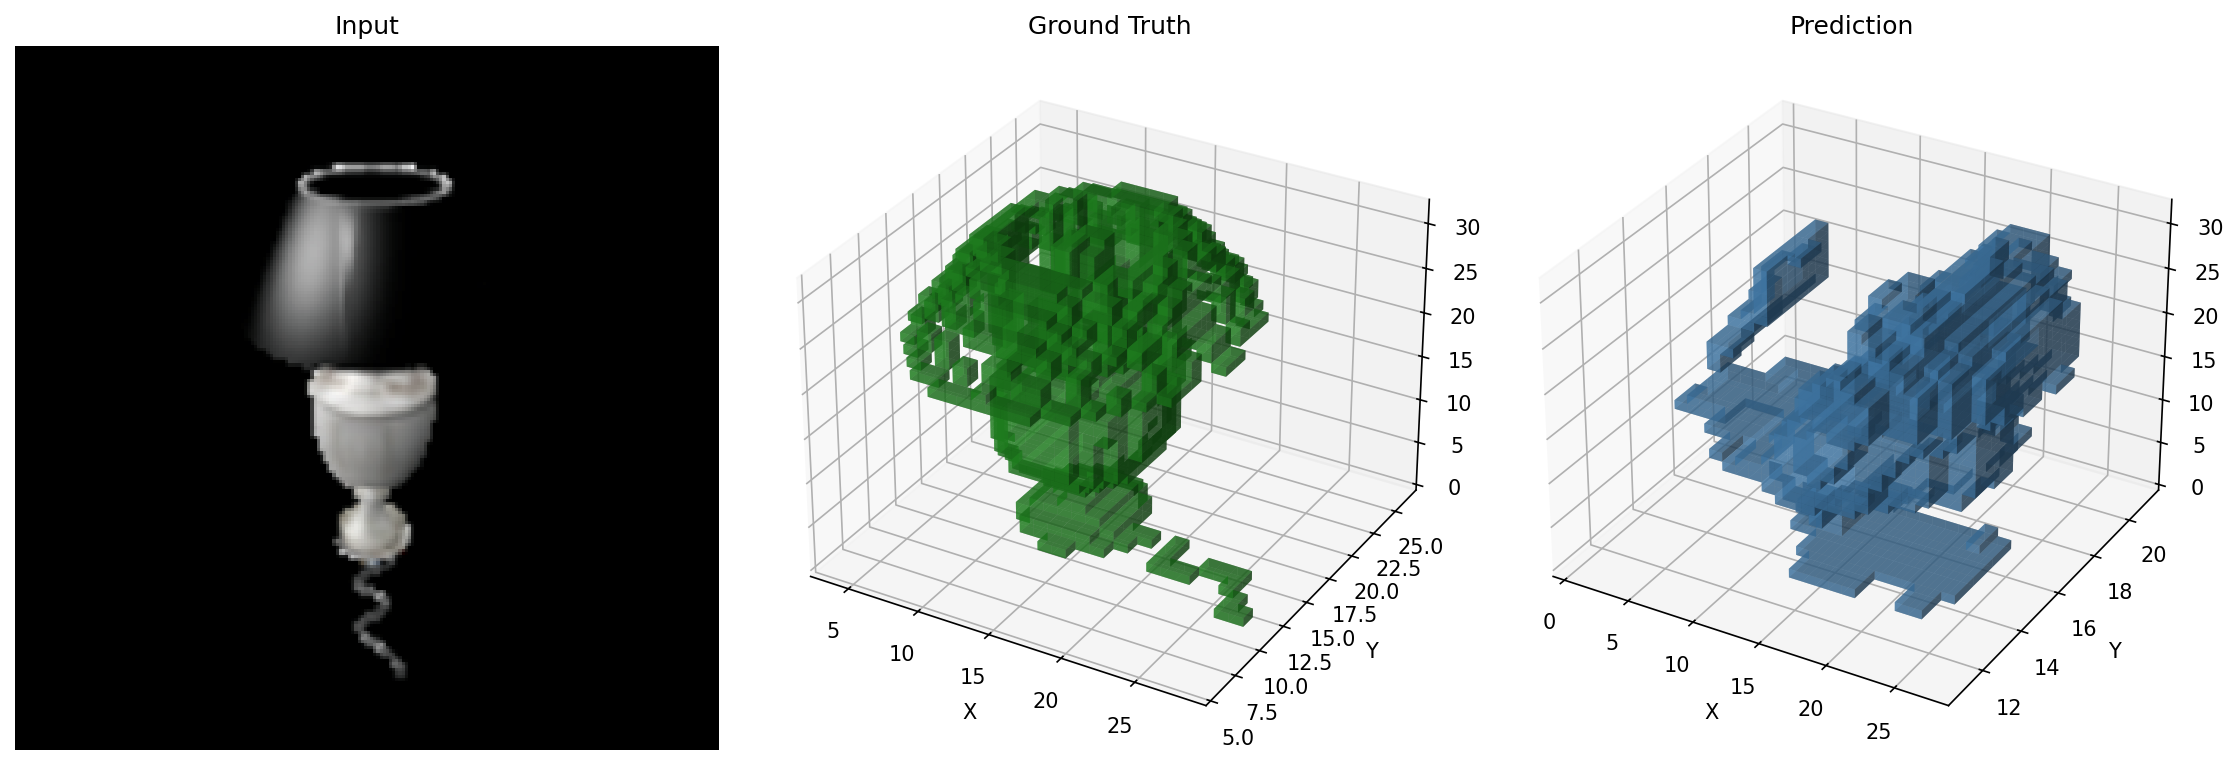
\includegraphics[width=0.32\textwidth]{plots/failure_lamp.png} &
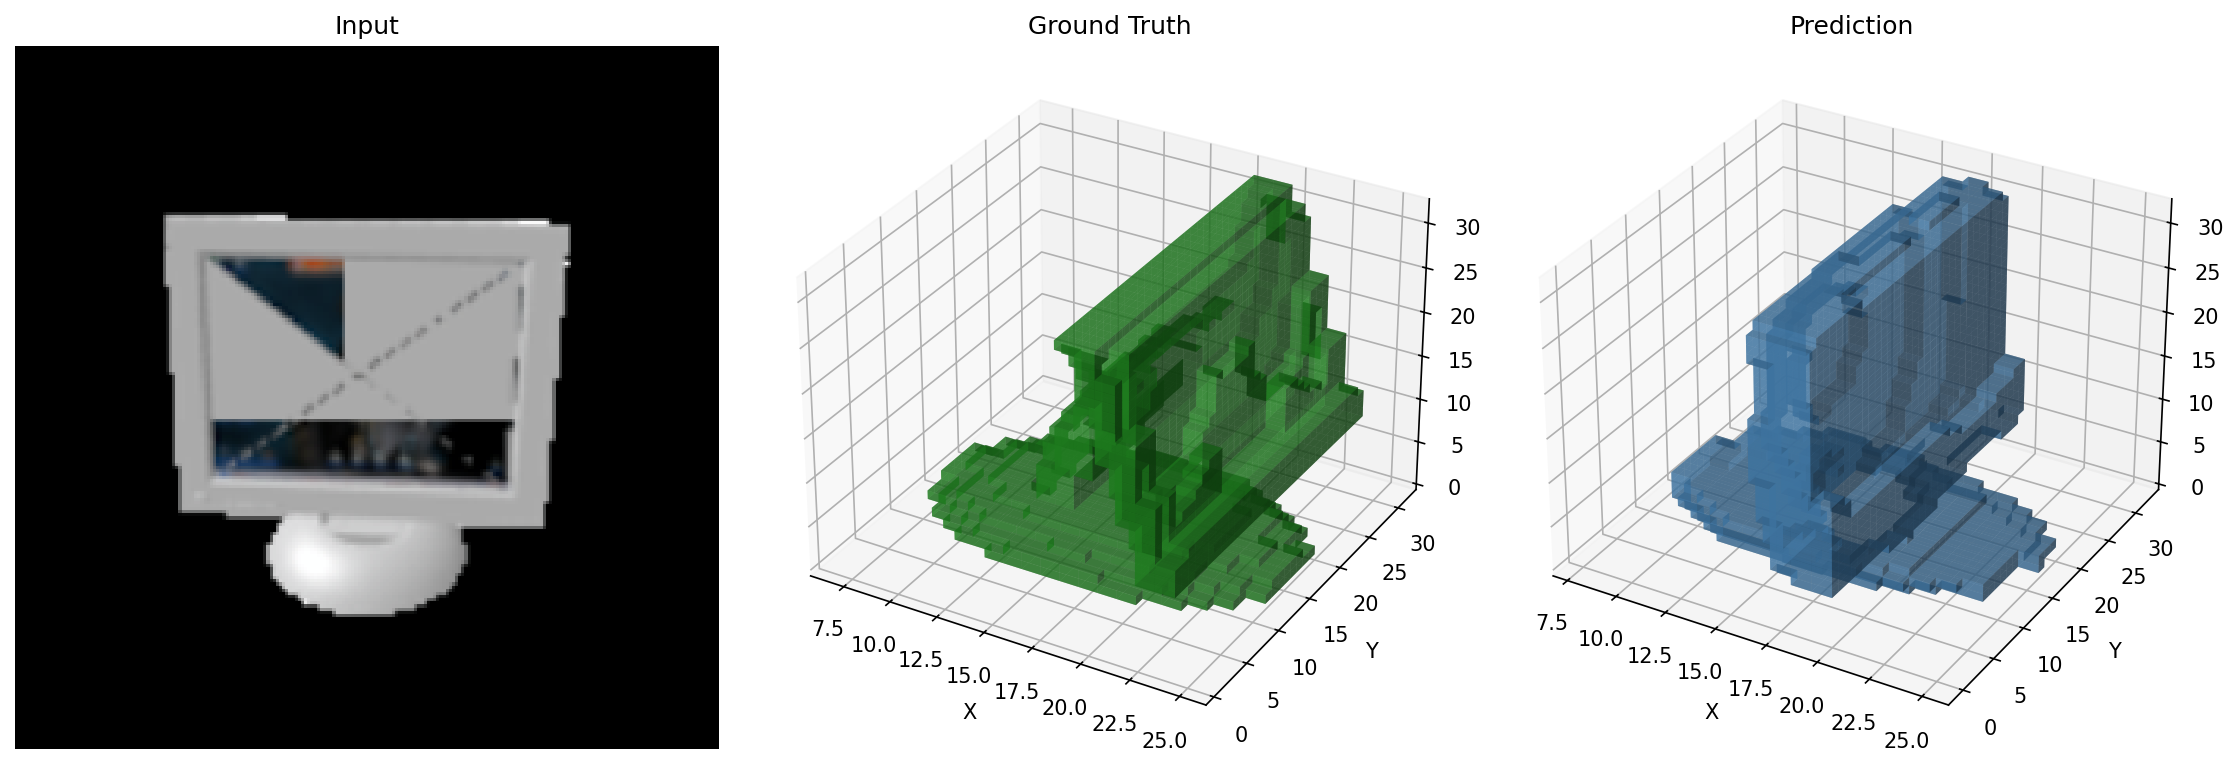
\includegraphics[width=0.32\textwidth]{plots/failure_display.png} &
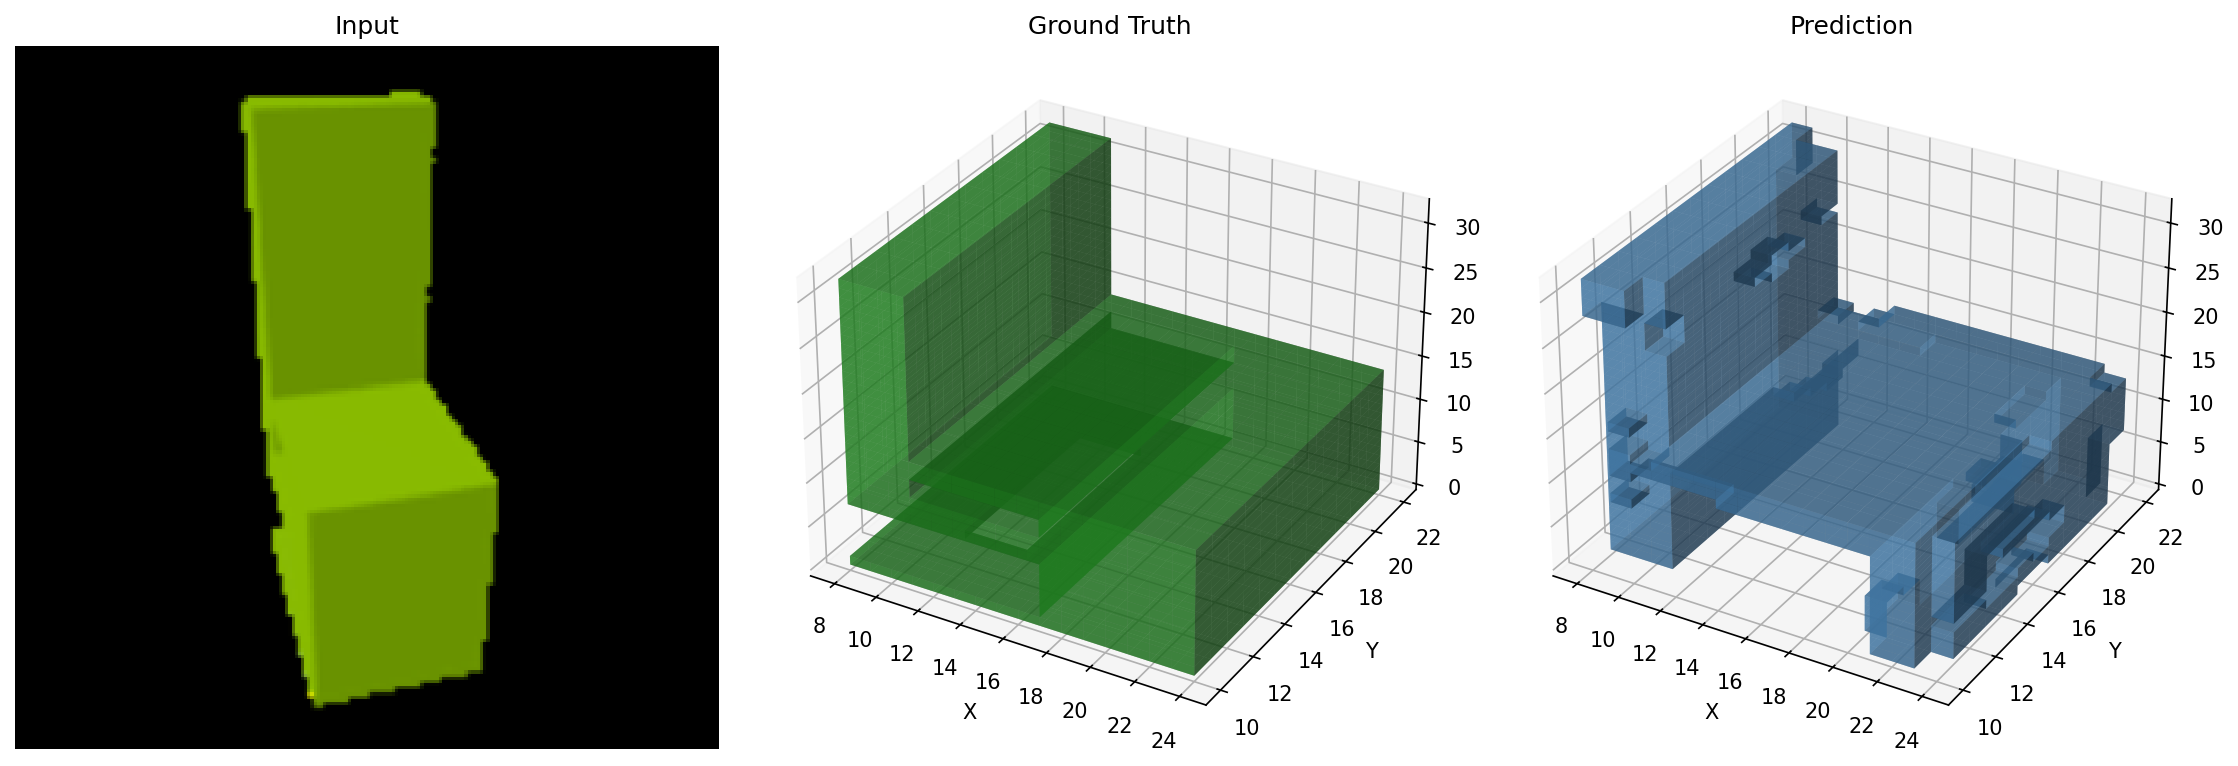
\includegraphics[width=0.32\textwidth]{plots/failure_chair.png} \\
(a) Lamp, IoU = 0.241 & (b) Display, IoU = 0.183 & (c) Chair, IoU = 0.552
\end{tabular}
\caption{Failure cases. Lamps and displays with thin structural elements (posts, stands, arms) are poorly reconstructed at $32^3$ resolution. The chair loses detail in the legs and armrests.}
\label{fig:failure}
\end{figure*}

% ============================================================
\section{Discussion}
\label{sec:discussion}
% ============================================================

\subsection{Simplifications and Assumptions}

Our approach makes several simplifying assumptions that are important to acknowledge:

\begin{itemize}
    \item \textbf{Single canonical object per image}: We assume each image contains exactly one centered object on a clean background. Real-world images with cluttered backgrounds, partial occlusions, or multiple objects would require additional preprocessing (detection, segmentation) before our model could be applied.
    \item \textbf{Fixed voxel resolution}: Our $32^3$ output grid provides a coarse approximation of 3D shape. Each voxel corresponds to roughly $1/32$ of the object's bounding box in each dimension, meaning features smaller than this scale are lost. This is a fundamental limitation of the voxel representation at this resolution.
    \item \textbf{Synthetic training data}: The ShapeNet rendered images are generated synthetically with controlled lighting, viewpoints, and clean backgrounds. The domain gap between these renderings and real photographs limits the model's applicability to real-world images without additional domain adaptation.
    \item \textbf{Category-agnostic model}: We train a single model across all 13 categories rather than category-specific models. While this is more general, category-specific models might achieve higher per-category performance by specializing their shape priors.
\end{itemize}

\subsection{Limitations and Future Work}

The most significant limitation of our approach is the voxel resolution. At $32^3$, thin structures like lamp posts, chair legs, and monitor stands cannot be faithfully represented. Increasing the resolution to $64^3$ or $128^3$ would improve geometric detail but at a cubic increase in memory and computation. Alternative representations could address this more efficiently:

\begin{itemize}
    \item \textbf{Octree representations}~\cite{tatarchenko2017octree} allocate resolution adaptively, spending more voxels near surfaces and fewer in empty regions.
    \item \textbf{Implicit functions}~\cite{mescheder2019occupancy,park2019deepsdf} can represent surfaces at arbitrary resolution by learning a continuous function that is sampled at query points during inference.
    \item \textbf{Mesh-based methods}~\cite{wang2018pixel2mesh} directly predict surface geometry, avoiding the discretization artifacts inherent to voxel grids.
\end{itemize}

Another limitation is the domain gap between synthetic renderings and real photographs. Future work could explore domain adaptation techniques, training on mixed real/synthetic data, or using self-supervised objectives that do not require 3D ground truth.

Had we continued this project, we would have explored several directions. First, increasing voxel resolution to $64^3$ with a deeper decoder would allow better representation of thin structures, though this would increase memory requirements by a factor of eight. Second, incorporating multi-view information when available could leverage the 3D-R2N2 paradigm of recurrent fusion or the Pix2Vox context-aware fusion to combine information from multiple viewpoints, substantially improving reconstruction quality. Third, using a feature pyramid network (FPN) in the encoder would preserve spatial information at multiple scales, potentially improving the decoder's ability to reconstruct objects with both large-scale structure and fine geometric detail. Fourth, training category-specific models could allow each model to develop specialized shape priors; for instance, a lamp-specific model might learn to hallucinate thin structural elements that a general model cannot. Fifth, incorporating 3D data augmentation such as random rotations and flips of the voxel grids during training could improve the model's robustness to viewpoint variation. Finally, exploring attention mechanisms in the decoder could allow the model to focus computational resources on the most informative regions of the voxel grid.

\subsection{Why BCE+Dice Outperforms Other Losses}

The strong performance of the combined BCE+Dice loss can be understood through the lens of class imbalance. In a typical $32^3$ voxel grid, only 2--5\% of voxels are occupied (as we observed in our data, with a mean occupancy ratio of approximately 0.024). BCE treats each voxel equally, meaning the gradient signal is dominated by the vast majority of empty voxels. The Dice component directly optimizes the overlap between predicted and ground-truth occupied regions, providing a complementary signal that is invariant to the number of background voxels.

Focal loss was designed to address a similar imbalance problem in object detection~\cite{lin2017focal}, but it performs poorly here. We hypothesize that this is because focal loss reduces the gradient magnitude for ``easy'' empty voxels, which are nonetheless important for learning accurate shape boundaries. In voxel reconstruction, the boundary voxels between occupied and empty regions carry the most important geometric information, and these are precisely the voxels that are neither ``easy'' occupied nor ``easy'' empty---they are the hardest examples. By reducing focus on the easy cases, focal loss may be degrading the learning signal for these critical boundary voxels.

\subsection{Comparison to Prior Work}

Our best result of 0.677 IoU compares favorably with established baselines on the ShapeNet benchmark. 3D-R2N2~\cite{choy2016r2n2} reported approximately 0.560 for single-view reconstruction, and Pix2Vox~\cite{xie2019pix2vox} reported approximately 0.661. While direct comparison requires caution due to potential differences in data splits, preprocessing, and evaluation protocols, our results demonstrate that a straightforward encoder-decoder with refinement can achieve competitive performance when combined with an appropriate loss function.

It is worth noting that our architecture is simpler than both 3D-R2N2 (which uses 3D convolutional LSTMs) and Pix2Vox (which includes a context-aware fusion module designed for multi-view aggregation). Our competitive results suggest that with modern pretrained encoders and careful loss function design, architectural complexity may be less important than previously believed for this task. This finding aligns with a broader trend in deep learning where well-tuned simple models often match or exceed more complex architectures, particularly when combined with effective training recipes. The fact that loss function selection (BCE+Dice) yields a larger improvement than doubling the encoder capacity (ResNet-18 to ResNet-50) is a practical insight: before scaling model size, practitioners should first optimize the training objective for their specific task characteristics.

\subsection{Ethical Considerations}

Following CVPR's Ethics Guidelines for Authors, we discuss the ethical implications of 3D reconstruction technology.

\paragraph{Privacy concerns.} 3D reconstruction from images raises privacy concerns, particularly when applied to scenes containing people or private spaces. A system that can reconstruct 3D environments from photographs could potentially be used for surveillance or to reconstruct private spaces without consent. While our work focuses on isolated object reconstruction from synthetic data, the underlying technology could be extended to more sensitive applications. Researchers should be mindful of these risks and consider implementing access controls, usage policies, and consent mechanisms when deploying such systems.

\paragraph{Dual use.} 3D reconstruction technology has legitimate applications in manufacturing, design, and accessibility, but it could also be misused for counterfeiting physical objects or creating unauthorized 3D replicas of copyrighted designs. As the fidelity of reconstruction methods improves, these risks become more significant.

\paragraph{Environmental impact.} Training deep learning models requires substantial computational resources. Our experiments used GPU hours on shared computing infrastructure. While the environmental impact of our specific experiments is modest (approximately 10 GPU-hours total), the broader trend of increasingly large models in computer vision warrants consideration of the carbon footprint of research.

\paragraph{Dataset biases.} ShapeNet, like many 3D model datasets, reflects the biases of its creators and sources. Certain object categories may be over-represented, and the 3D models may reflect cultural biases in design aesthetics. Models trained on such data may perform poorly on objects from underrepresented cultures or design traditions.

\paragraph{Data provenance.} The ShapeNet dataset consists of 3D models sourced from online repositories. While the dataset curators obtained appropriate permissions, the broader practice of scraping 3D models from the internet raises questions about creator consent and attribution that the community should continue to address.

% ============================================================
\section{Conclusion}
\label{sec:conclusion}
% ============================================================

We have presented a single-image 3D reconstruction system that predicts $32 \times 32 \times 32$ voxel occupancy grids from RGB images using an encoder-decoder architecture with optional residual refinement. Through systematic experiments on the ShapeNet/R2N2 benchmark, we identified several key findings:

First, the choice of loss function has a significant impact on reconstruction quality. The combined BCE+Dice loss outperforms all other configurations, including pure BCE, focal loss, and a larger ResNet-50 encoder with BCE. This demonstrates that addressing the inherent class imbalance in voxel prediction is more important than increasing model capacity.

Second, the residual refinement module provides consistent improvements with minimal additional parameters, confirming the value of a dedicated post-processing stage for correcting coarse decoder outputs.

Third, our per-category analysis reveals a clear relationship between object geometry and reconstruction difficulty. Compact, convex objects (cars, cabinets, telephones) are reconstructed with high fidelity (IoU $>$ 0.80), while objects with thin structures or high shape diversity (lamps, displays) remain challenging (IoU $<$ 0.55). This limitation is fundamentally tied to the $32^3$ voxel resolution and motivates future exploration of higher-resolution or continuous 3D representations.

Our best model achieves a test IoU of 0.677, competitive with established methods such as 3D-R2N2 (0.560) and Pix2Vox (0.661), despite using a simpler architecture. This suggests that careful engineering of loss functions and training procedures can compensate for architectural simplicity in single-image 3D reconstruction. Looking forward, we believe the insights from our ablation studies---particularly the importance of loss function design for class-imbalanced voxel prediction---generalize beyond our specific architecture and could benefit researchers working on related 3D prediction tasks, including semantic scene completion, occupancy prediction for autonomous driving, and medical volumetric segmentation.

% ============================================================
\section*{Individual Contributions}
% ============================================================

\textbf{Angelina Quan}: Implemented the training and evaluation pipeline, including the dataset loader, loss functions, and metrics. Designed and ran all ablation experiments. Wrote the Methodology, Experimental Results, and Discussion sections of the paper. Generated all visualizations and failure case analysis.

\textbf{[Partner Name]}: [Describe partner's contributions here---e.g., implemented the model architecture, conducted related work survey, wrote Introduction and Related Work sections, helped with experimental design and paper editing.]

% ============================================================
\section*{Use of Generative AI Tools}
% ============================================================

We used Cursor (Claude) as a generative AI coding assistant for the following tasks:
\begin{itemize}
    \item Writing boilerplate code for the data loader, model architecture, and training loop.
    \item Generating SLURM job submission scripts for the computing cluster.
    \item Assisting with debugging and code organization.
    \item Drafting sections of this report, which were then reviewed and edited by the authors.
\end{itemize}

All experimental design decisions, analysis, and interpretation of results were performed by the authors. The AI tool was used as a productivity aid, not as a substitute for understanding or intellectual contribution.

{\small
\bibliographystyle{ieee_fullname}
\bibliography{refs}
}

\end{document}
